% UQ ability vs cost: current foundation-compare contenders
% Upload this single file to Overleaf (TeX Live 2022+). Compile with pdfLaTeX.
\documentclass[11pt,a4paper]{article}

\usepackage[margin=1in]{geometry}
\usepackage{amsmath,amssymb,amsthm,bm,mathtools}
\usepackage{booktabs,tabularx,enumitem,microtype,xcolor,hyperref}
\usepackage{tikz}
\usetikzlibrary{arrows.meta,positioning,fit,calc}

\hypersetup{colorlinks=true,linkcolor=blue!50!black,citecolor=blue!50!black,urlcolor=blue!60!black}

\theoremstyle{definition}
\newtheorem{definition}{Definition}
\newtheorem{remark}{Remark}

\newcommand{\R}{\mathbb{R}}
\newcommand{\E}{\mathbb{E}}
\newcommand{\Var}{\mathrm{Var}}
\newcommand{\Ncal}{\mathcal{N}}
\newcommand{\GP}{\mathcal{GP}}
\newcommand{\D}{\mathcal{D}}
\newcommand{\softplus}{\operatorname{softplus}}
\newcommand{\sigmoid}{\operatorname{sigmoid}}
\newcommand{\Kmax}{K_{\max}}
\newcommand{\Keff}{K_{\mathrm{eff}}}

\title{\textbf{Uncertainty Quantification vs.\ Cost}\\[0.35em]
\large Best Contenders in the SpectralGPPlus Foundation Compare\\[0.25em]
\normalsize Derivations, Feature Catalog, and Empirical Ranking}
\author{SpectralGPPlus \,/\, \texttt{experiments\_MOEGP/feasibility\_mode\_count}\\
Companion to \texttt{gamma\_mlp\_hist\_mogp\_analysis.md} (Tiers~1--4)}
\date{\today}

\begin{document}
\maketitle

\begin{abstract}
We analyze the models currently under test in the foundation-model comparison
harness by \emph{uncertainty-quantification (UQ) ability} and \emph{wall-clock
cost}. TabPFN-3.5 remains the pretrained ceiling on negative log score.
Among classical (non-pretrained) methods, three regimes emerge on the
UQ--cost Pareto front: (i)~a logistic Gaussian-process density
(\texttt{logistic\_gp} / \texttt{logistic\_gp\_sorf\_map}) for calibrated
densities at $\sim$4--25\,s; (ii)~a pinball quantile GP
(\texttt{quantile\_gp\_*} / SORF hybrids) for CRPS at $\sim$4--50\,s; and
(iii)~calibrated MidlineSparse gamma mixtures
(\texttt{midline\_gamma\_mlp\_t1} / lean auto) for interpretable
co-located multimodality at $\sim$2--3\,min.
Histogram Kronecker MoGP (\texttt{hist\_mogp\_t1}) is a controlled
TabPFN-interface baseline, not the UQ winner after Tier~3.
This note derives each method as implemented, enumerates every feature added
across Tiers~1--4, and ranks contenders with three-seed means from
\texttt{results/foundation\_compare\_tier\{1,3,4\}/}.
\end{abstract}

\tableofcontents
\newpage

%==============================================================================
\section{Protocol and metrics}
\label{sec:protocol}
%==============================================================================

\subsection{Problems and splits}
Synthetic suite (unless noted $n_{\mathrm{train}}=100$, $n_{\mathrm{test}}=200$):
\textbf{A01} (co-located bimodal), \textbf{unimodal}, \textbf{A02} ($x$-separated
step), \textbf{A04} (co-located trimodal), \textbf{A05}, \textbf{A06}
(heteroscedastic lognormal noise).
Tabular: QSAR fish ($n{=}726/182$, $d{=}6$) and TabArena concrete
($n{=}824/206$, $d{=}8$). Seeds $\{0,1,42\}$; Tier~4 also reports fresh
seeds $\{3,4,5\}$ and large-$n$ synthetics ($n\in\{1000,5000\}$).

\subsection{UQ metrics}
\begin{itemize}[leftmargin=1.4em,itemsep=0.15em]
  \item \textbf{Negative log score} (mean NLL of the predictive density): primary
        proper scoring rule for densities.
  \item \textbf{CRPS}: continuous ranked probability score. For mixtures we use
        the Grimit et al.\ closed form; for bar / histogram PPDs we use exact
        piecewise-uniform bar CRPS (\texttt{CRPS\_bar} / \texttt{CRPS exact}).
        The ScoringBench moment-summary CRPS misrepresents heavy-tailed bars.
  \item \textbf{cov90}: empirical coverage of central 90\% predictive intervals
        (nominal $0.90$).
  \item \textbf{Hellinger}: mean Hellinger distance to the true conditional
        density at probe points (synthetics with known $p^\star$ only).
  \item \textbf{RMSE}: point accuracy of the predictive mean (ceiling set by
        Stage~1 for midline models).
\end{itemize}

\subsection{Cost}
Primary cost is wall-clock fit$+$predict time \texttt{wall\_s} stamped by the
adapters / compare harness (CPU/GPU environment of
\texttt{gpplus2026}). Secondary costs (memory, FLOPs) are not ranked here.
Reported times are pessimistic under multi-process Tier runs.

%==============================================================================
\section{Models currently under test}
\label{sec:roster}
%==============================================================================

\begin{center}
\renewcommand{\arraystretch}{1.08}
\small
\begin{tabular}{@{}llp{6.6cm}@{}}
\toprule
Key family & Role & Status \\
\midrule
\texttt{tabpfn35} & TabPFN-3.5 bar PPD & FM ceiling \\
\texttt{tabpfn3}, \texttt{kumo}, \texttt{tabgp} & Other FMs & Baselines \\
\texttt{exact\_gp}, \texttt{ni\_sorf} & Unimodal GP / SORF & Baselines \\
\texttt{mdn}, \texttt{mdn\_const} & Bishop MDN & Estimative MoG controls \\
\texttt{midline}, \texttt{midline\_gamma\_mlp} & MidlineSparse MoG & Structure champion \\
\texttt{midline\_*\_mogp} & Residual / Bayes MoGP & Sibling UQ objects \\
\texttt{midline\_gamma\_mlp\_t1/het/auto*} & Calibrated / auto gamma & Active contenders \\
\texttt{hist\_mogp\_t1} & Kronecker hist MoGP & Bar-interface control \\
\texttt{logistic\_gp[\_sorf\_*]} & Logistic-GP density & Density Pareto winner \\
\texttt{quantile\_gp[\_sorf/hybrid*]} & Quantile + GPD tails & CRPS Pareto winner \\
\texttt{hist\_gpd*}, \texttt{hist\_lmc*}, \texttt{*\_vexp} & Ablations & Deprecated defaults \\
\bottomrule
\end{tabular}
\end{center}

\paragraph{Active classical contenders.}
\texttt{logistic\_gp} / \texttt{logistic\_gp\_sorf\_map},
\texttt{quantile\_gp\_indep} / \texttt{quantile\_gp\_sorf} / \texttt{\_hybrid\_auto},
\texttt{midline\_gamma\_mlp\_t1} and lean auto (\texttt{\_1mid} / \texttt{\_c85}),
\texttt{hist\_mogp\_t1} as audit baseline.

%==============================================================================
\section{Method derivations}
\label{sec:derivations}
%==============================================================================

\subsection{MidlineSparse gamma mixture (Stage 1--2)}
\label{sec:gamma}

\paragraph{Problem class.}
Co-located multimodality: modes of $p(y\mid x)$ are \emph{not} encoded by an
$x$-gate. A02 (step) is the stress case where that assumption fails.

\paragraph{Stage 1 (midline).}
Exact GP (or LOO / padded-SORF Bayesian linear core) on all $n$ points:
\begin{equation}
  y = f_0(x)+\varepsilon,\qquad
  f_0\sim\GP\bigl(m(\cdot),k(\cdot,\cdot)\bigr).
\end{equation}
Predictive midline $(\mu_0(x),\sigma_0(x))$ is frozen. Optional cap
\begin{equation}
  \sigma_0^{\mathrm{mix}}(x)
  =
  \min\bigl(\sigma_0(x),\,\max(c\,\widehat{\mathrm{Std}}(y-\mu_0),\,0.05)\bigr),
\end{equation}
with $c=\texttt{std0\_cap\_frac}$ (default $0.3$). LOO Stage~1 replaces
in-sample residuals by closed-form leave-one-out predictives so Stage~2 does
not train on overfit Stage-1 fits.

\paragraph{Stage 2 (sparse MoG on residuals).}
Overcomplete budget $\Kmax$. Hard-Concrete switches $\alpha_k\in[0,1]$,
gates $\pi(x)\in\Delta^{\Kmax-1}$, offsets $\delta_k(x)$, carve-out
$\gamma_k(x)\in(0,1)$ (constant or MLP):
\begin{align}
  \mu_k(x)
  &=
  \mu_0(x)+\alpha_k\,\delta_k(x),
  \\
  \mathrm{Var}_k(x)
  &=
  \bigl[\sigma_0^{\mathrm{mix}}(x)\bigr]^2\,
  \bigl(1-\alpha_k\gamma_k(x)\bigr)\,\beta_k
  +\varepsilon.
\end{align}
Champion settings use $\beta_k\equiv 1$. Predictive density
\begin{equation}
  p_\theta(y\mid x)
  =
  \sum_{k=1}^{\Kmax}
  \pi_k(x)\,
  \Ncal\!\bigl(y;\,\mu_k(x),\,\mathrm{Var}_k(x)\bigr).
\end{equation}
Training maximizes mixture log-likelihood minus Hard-Concrete $L_0$ complexity
and optional usage / merge controllers. The fitted object is an
\emph{estimative} mixture of Gaussians (EB--MAP), not a Bayesian posterior
predictive~\cite{foundations-note}.

\paragraph{Hard-Concrete (Louizos et al.).}
With stretch $(\gamma_{\mathrm{HC}},\zeta_{\mathrm{HC}})=(-0.1,1.1)$ and
temperature $\beta_{\mathrm{HC}}=2/3$,
\begin{equation}
  \alpha_k
  =
  \mathrm{clip}_{[0,1]}
  \bigl(
    \sigmoid(\log\alpha_k)\,(\zeta_{\mathrm{HC}}-\gamma_{\mathrm{HC}})
    +\gamma_{\mathrm{HC}}
  \bigr)
\end{equation}
(deterministic eval); stochastic Concrete reparameterization during training;
complexity $\sum_k \sigmoid(\log\alpha_k-\beta_{\mathrm{HC}}\log t)$ with
$t=-\gamma_{\mathrm{HC}}/\zeta_{\mathrm{HC}}$.

\begin{figure}[ht]
\centering
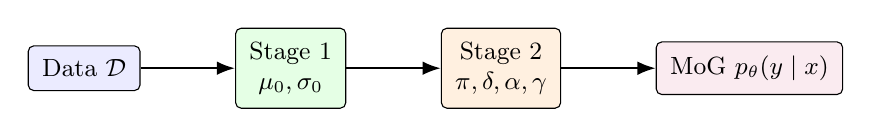
\begin{tikzpicture}[
  box/.style={draw,rounded corners=2pt,align=center,inner sep=5pt,font=\small},
  arr/.style={-{Latex},thick}
]
\node[box,fill=blue!8] (d) {Data $\D$};
\node[box,fill=green!10,right=1.2cm of d] (s1) {Stage~1\\ $\mu_0,\sigma_0$};
\node[box,fill=orange!12,right=1.2cm of s1] (s2) {Stage~2\\ $\pi,\delta,\alpha,\gamma$};
\node[box,fill=purple!8,right=1.2cm of s2] (p) {MoG $p_\theta(y\mid x)$};
\draw[arr] (d)--(s1);\draw[arr] (s1)--(s2);\draw[arr] (s2)--(p);
\end{tikzpicture}
\caption{MidlineSparse two-stage pipeline.}
\label{fig:gamma-pipe}
\end{figure}

\subsection{Histogram Kronecker MoGP}
\label{sec:hist}

Partition the response into $B$ bins with borders $\{b_j\}$ (equal-width preferred;
optional outer tails of width $\texttt{tail\_frac}\times\mathrm{span}$).
Encode training labels as one-hot $H\in\{0,1\}^{n\times B}$ and place a
multi-output GP with separable Kronecker kernel
\begin{equation}
  \mathrm{Cov}\bigl(\mathrm{vec}(F)\bigr)
  =
  K_{XX}\otimes K_{HH}
\end{equation}
under a Gaussian likelihood on $H$. Posterior mean $\widehat F(x)\in\R^B$ is
projected onto the simplex (Euclidean projection) to obtain bar masses
$\pi_b(x)$; density on bin $b$ is $\pi_b(x)/w_b$.

\paragraph{Degeneracy-safe eigh.}
Tail bins make $K_{HH}$ nearly block-identity with repeated eigenvalues.
Stock $\texttt{torch.linalg.eigh}$ backward divides by $\lambda_j-\lambda_i$;
\texttt{\_SafeEigh} zeroes near-degenerate gap terms (exact for log-det /
quadratic forms).

\paragraph{Dirichlet-GP variant (\texttt{hist\_gpd}).}
Milios-style classification likelihood on bin indices with fixed empty-bin
class count; softmax-MC averaging optional. Empirically dominated by
\texttt{hist\_mogp\_t1} on CRPS and most log scores.

\subsection{Logistic-GP conditional density}
\label{sec:logistic}

\paragraph{Object.}
This is the continuous / soft analogue of TabPFN's bar interface: a
\emph{conditional density} on a fixed $y$-grid, not an inverse-CDF model.
On cell centres $\{y_g\}_{g=1}^{G}$ with widths $w_g$ (default $G{=}128$ inner
cells plus two wide outer tail cells),
\begin{equation}
  p(y\in\mathrm{cell}_g\mid x)
  =
  \pi_g(x),
  \qquad
  \pi(x)=\mathrm{softmax}\bigl(f(x,y_\cdot)+\log w_\cdot\bigr)\in\Delta^{G-1}.
\end{equation}
The continuous density inside a cell is $\pi_g(x)/w_g$. The latent field is a
logistic Gaussian process density~\cite{tokdar2010}:
$p(y\mid x)\propto\exp f(x,y)$, discretized by the softmax over cells.

\paragraph{Latent field (v1 RFF / v2 SORF).}
Write $r=y-m(x)$ and decompose
\begin{equation}
  f(x,y)
  =
  \underbrace{-\tfrac12\bigl(r/s(x)\bigr)^2-\log s(x)}_{\text{Gaussian base}}
  +
  \underbrace{\beta(y)}_{\text{marginal RW}}
  +
  \underbrace{f_{\mathrm{GP}}(x,r)}_{\text{RFF/SORF shape}}.
\end{equation}
The base prevents a knife-edge ridge $y\approx m(x)$ from forcing
$\ell_y\to 0$. The vector $\beta\in\R^G$ has a second-difference
(random-walk) Gaussian prior and carries $x$-independent structure (e.g.\ the
two levels of A02). The shape term is a GP on $(x,r)$ with separable RBF
covariance, approximated by random features.

\paragraph{Separable kernel vs.\ Kronecker (what is / is not Kronecker here).}
A stationary RBF on the product space factorizes in frequency:
\begin{equation}
  k\bigl((x,r),(x',r')\bigr)
  =
  k_x(x,x')\,k_r(r,r')
  \;\approx\;
  \phi(x,r)^\top\phi(x',r').
\end{equation}
On a Cartesian grid of inputs $\times$ $y$-cells this induces a covariance that
\emph{would} be Kronecker-structured if we stored $\mathrm{vec}(F)$ as an
exact GP (as \texttt{hist\_mogp} does with $K_{XX}\otimes K_{HH}$).
The logistic model does \emph{not} form or invert that Kronecker matrix.
Instead it uses the trigonometric factorization of the feature map.
With frequencies $(\omega_x,\omega_y)$ and phases folded into
$a(x)=\omega_x^\top x/\ell_x-\omega_y m(x)/\ell_y$,
$c_g=\omega_y y_g/\ell_y$,
\begin{equation}
  \cos(a_d+c_{gd})
  =
  \cos a_d\cos c_{gd}-\sin a_d\sin c_{gd},
\end{equation}
so
\begin{equation}
  f_{\mathrm{GP}}(x,y_g)
  =
  \frac{\sigma_f}{\sqrt{D}}
  \sum_{d=1}^{D}
  \bigl(
    w_{c,d}\cos(a_d+c_{gd})
    +
    w_{s,d}\sin(a_d+c_{gd})
  \bigr)
\end{equation}
is two products of size $[N,D]\times[D,G]$---never an $[N,G,D]$ tensor and never
a Kronecker solve. (Hist-MoGP's $K_{XX}\otimes K_{HH}$ is the same
\emph{separable} modelling idea, with a different likelihood and an exact
eigh-based GP step.)

\paragraph{Likelihood / training loss.}
Training labels are cell indices $g_i=\mathrm{bin}(y_i)$. The proper scoring
rule is the continuous log density on the occupied cell,
\begin{equation}
  \ell_i
  =
  -\log\bigl(\pi_{g_i}(x_i)/w_{g_i}\bigr)
  =
  -\log\pi_{g_i}(x_i)+\log w_{g_i},
\end{equation}
i.e.\ categorical NLL of the softmax probabilities, corrected by bin width so
the score matches $\int p(y\mid x)\,dy$ rather than discrete cell mass.
With a fixed 15\% calibration mask $\mathcal{C}$ and fit set $\mathcal{F}$,
\begin{align}
  \mathcal{L}
  &=
  \frac{1}{|\mathcal{F}|}
  \Bigl(
    \sum_{i\in\mathcal{F}}\ell_i
    +
    \tfrac12\|w\|^2
    +
    \tfrac12\|v_m\|^2
    +
    \tfrac12\|v_s\|^2
    +
    \tfrac12\|D_2\beta/\varsigma\|^2
  \Bigr)
  \nonumber\\
  &\quad
  +
  \frac{1}{|\mathcal{C}|}\sum_{i\in\mathcal{C}}\ell_i\Big|_{w\,\mathrm{detached}}.
\end{align}
Weights / base coefficients are trained on $\mathcal{F}$; lengthscales and the
$\varepsilon$-floor see gradients only from $\mathcal{C}$ (detached $w$),
matching the auto-gamma in-loop calibration pattern. A mixture floor
$(1-\varepsilon)\pi+\varepsilon m_{\mathrm{train}}$ keeps cells off numerical
zero. Default inference is \textbf{MAP} on $w$; mean-field VI was strictly
worse (Tier~4).

\paragraph{Why this loss matches log score.}
Evaluation log score is exactly the same continuous NLL on test cells.
CRPS is computed afterwards from the bar PPD (exact piecewise-uniform CRPS),
not optimized directly---so logistic-GP wins density metrics more than CRPS.

\subsection{Quantile GP with GPD tails}
\label{sec:quantile}

\paragraph{Object.}
The dual of logistic / TabPFN bars: instead of ``mass on a $y$-grid'', predict
the \emph{inverse} CDF---the numbers $q(x,\tau)$ such that
$P(Y\le q(x,\tau)\mid x)=\tau$---at fixed probabilities
$\tau_1<\cdots<\tau_J$ (default $J{=}19$)~\cite{abeywardana2015}.
Example: $\tau{=}0.5$ is the median; $\tau{=}0.9$ is the 90th percentile.

\paragraph{Why ``monotone softplus increments''?}
A CDF inverse must be nondecreasing in $\tau$: higher probability $\Rightarrow$
higher or equal $y$. If you fit each $\tau$ with a separate unrestricted head,
nothing stops
$q(x,0.9)<q(x,0.5)$ (``crossing quantiles''), which is nonsense as a CDF.

\texttt{softplus}$(z)=\log(1+e^{z})$ is a smooth map $\R\to(0,\infty)$
(always positive; like a soft $\mathrm{ReLU}$). So build the quantile curve
by \emph{starting low and only adding positive gaps}:
\begin{align}
  q(x,\tau_1)
  &=
  f_0(x)
  &&
  \text{(unrestricted location of the lowest knot),}
  \\
  q(x,\tau_{j+1})
  &=
  q(x,\tau_j)
  +
  \underbrace{\softplus\bigl(f_j(x)\bigr)}_{\text{always }>0}
  +\varepsilon.
\end{align}
Whatever raw scores $f_j(x)=h(x)^\top W_{:,j}+c_j$ the network outputs, the
\emph{gaps} stay positive, so
$q(x,\tau_1)<q(x,\tau_2)<\cdots<q(x,\tau_J)$ automatically.
That construction is ``monotone softplus increments''.
(The \texttt{indep} variant skips this and fits each $\tau$ freely, then sorts
at predict time.)

\paragraph{Kronecker prior --- plain meaning.}
The weight matrix $W_{\mathrm{inc}}\in\R^{p\times(J-1)}$ has
\begin{itemize}[leftmargin=1.2em,itemsep=0.1em]
  \item \textbf{rows} $=$ feature coordinates of the RFF/SORF map $h(x)$,
  \item \textbf{columns} $=$ successive $\tau$-gaps.
\end{itemize}
We want nearby $\tau$-levels to share similar weights (smooth quantile shape),
but different feature coordinates to be independent a priori. That is:
each row is a smooth Gaussian path over $\tau$, and rows do not talk to each
other. If $K_\tau$ is an RBF kernel on the gap indices, that prior is written
compactly as
\begin{equation}
  \mathrm{vec}_r(W_{\mathrm{inc}})
  \;\sim\;
  \Ncal\!\bigl(0,\; I_p\otimes K_\tau\bigr)
\end{equation}
(``$I_p\otimes K_\tau$'' $=$ block-diagonal with $p$ copies of $K_\tau$).

\paragraph{What the ``Frobenius quadratic'' is.}
For a Gaussian $\Ncal(0,\Sigma)$, the negative log-density is
$\tfrac12 v^\top\Sigma^{-1}v$ (plus constants). Here $v$ is all entries of
$W_{\mathrm{inc}}$ and $\Sigma=I_p\otimes K_\tau$, so
$\Sigma^{-1}=I_p\otimes K_\tau^{-1}$. Expanding the quadratic gives one
Mahalanobis penalty \emph{per row}:
\begin{equation}
  \tfrac12\sum_{i=1}^{p}
  \underbrace{
    w_{i,\cdot}\,K_\tau^{-1}\,w_{i,\cdot}^\top
  }_{\text{``how rough is feature $i$'s path over $\tau$?''}}.
\end{equation}
``Frobenius'' just means summing those row penalties over the whole matrix
(the matrix analogue of $\|W\|_F^2=\sum_{ij}W_{ij}^2$, but with $K_\tau^{-1}$
mixing the $\tau$-columns). In code it is
\texttt{(W @ K\_inv * W).sum()}. Intuition: if two adjacent $\tau$-columns of
$W$ differ a lot, the prior pays; if they are similar, the prior is happy.
The lowest-quantile column $W_{:,0}$ uses a plain $\tfrac12\|W_{:,0}\|^2$
ridge instead.

\paragraph{Pinball loss --- what it actually means.}
Fix one level $\tau\in(0,1)$ and a guess $q$ for the $\tau$-quantile of $Y$.
The residual is $u=y-q$. Pinball (``check'') loss is the asymmetric absolute
error
\begin{equation}
  \rho_\tau(u)
  =
  \begin{cases}
    \tau\,|u| & \text{if } y\ge q \quad (u\ge 0:\text{ underprediction}),\\
    (1-\tau)\,|u| & \text{if } y< q \quad (u<0:\text{ overprediction}).
  \end{cases}
\end{equation}
Equivalently $\rho_\tau(u)=\max(\tau u,\,(\tau-1)u)$.

\textit{Concrete example.} $\tau{=}0.9$, true $y{=}10$.
\begin{itemize}[leftmargin=1.2em,itemsep=0.1em]
  \item Guess $q{=}8$ (too low): pay $0.9\cdot 2=1.8$.
  \item Guess $q{=}12$ (too high): pay $0.1\cdot 2=0.2$.
\end{itemize}
Underpredicting a high quantile is expensive; overpredicting it is cheap.
For $\tau{=}0.1$ the asymmetry flips. For $\tau{=}0.5$,
$\rho_{1/2}(u)=\tfrac12|u|$ (ordinary absolute error / median regression).

\paragraph{Why pinball finds the true quantile.}
The expected pinball $\E[\rho_\tau(Y-q)]$ is minimized (uniquely, under mild
conditions) exactly when $q$ is the $\tau$-quantile of $Y$. So gradient
descent on pinball is not an ad-hoc ranking loss---it is the proper scoring
rule for a single quantile. The asymmetric Laplace likelihood is the same
thing in probabilistic clothing:
$-\log p_{\mathrm{ALD}}(y\mid q,\sigma)=\log\sigma+\rho_\tau(y-q)/\sigma+\mathrm{const}$;
the learned $\sigma$ only balances data fit against the Kronecker prior.

\paragraph{Link to CRPS.}
The continuous ranked probability score of a predictive CDF satisfies
\begin{equation}
  \mathrm{CRPS}(F,y)
  =
  2\int_0^1 \rho_\tau\bigl(y-F^{-1}(\tau)\bigr)\,d\tau.
\end{equation}
So averaging pinball over a dense $\tau$-grid \emph{is} a discrete CRPS.
That is the operational reason the quantile GP is the CRPS specialist, while
logistic-GP (density NLL) is the log-score specialist.

\paragraph{Full training loss (as implemented).}
With fit set $\mathcal{F}$, calib mask $\mathcal{C}$, and optional hybrid
weight $\lambda\ge 0$,
\begin{align}
  \mathcal{L}
  &=
  \frac{1}{|\mathcal{F}|}
  \Biggl(
    \sum_{i\in\mathcal{F}}\sum_{j=1}^{J}
      \frac{\rho_{\tau_j}\bigl(y_i-q(x_i,\tau_j)\bigr)}{\sigma}
    +
    |\mathcal{F}|\,J\log\sigma
    +
    \mathrm{prior}(W)
  \Biggr)
  \nonumber\\
  &\quad
  +
  \lambda\cdot
  \frac{1}{|\mathcal{F}|}
  \sum_{i\in\mathcal{F}}
  \bigl(-\log p_{\mathrm{knot}}(y_i\mid q(x_i,\cdot))\bigr)
  \nonumber\\
  &\quad
  +
  \frac{J}{|\mathcal{C}|}
  \sum_{i\in\mathcal{C}}
  \overline{\rho}\bigl(y_i,q(x_i,\cdot)\bigr)\Big|_{W\,\mathrm{detached}}.
\end{align}
Here $p_{\mathrm{knot}}$ is the piecewise-uniform density implied by the knots,
$\Delta\tau_j/(q_{j+1}-q_j)$ on the interior (plus provisional exponential
tails for a differentiable training NLL). The learned $\sigma$ balances
pinball against the Kronecker prior. Lengthscales are updated from $\mathcal{C}$
only. For $\lambda=\texttt{"auto"}$, a small grid $\{0,0.1,1\}$ is scored by
held-out $\overline{\rho}\cdot J+(-\log p_{\mathrm{knot}})$.

\paragraph{Predictive density and GPD tails.}
After fitting, outer tails use a generalized Pareto distribution with scale
$\kappa$ and shape $\xi$ chosen by training-row likelihood (replacing the
training exponential). Between knots the density remains
$\Delta\tau/\Delta q$, which spikes when adjacent quantiles collide---hence
strong CRPS but fragile log score unless hybrid $\lambda>0$ is selected.

\paragraph{Logistic vs.\ quantile vs.\ hist Kronecker (summary).}
\begin{center}
\renewcommand{\arraystretch}{1.08}
\small
\begin{tabular}{@{}p{2.4cm}p{3.6cm}p{3.8cm}@{}}
\toprule
 & Parameterization & Kronecker role \\
\midrule
\texttt{hist\_mogp} &
  bar masses via MOGP on one-hots &
  exact $K_{XX}\otimes K_{HH}$ GP solve \\
\texttt{logistic\_gp} &
  $\mathrm{softmax}\,f(x,y)$ on $y$-grid &
  separable $k_x k_y$ via RFF/SORF
  factorization; \emph{no} Kronecker invert \\
\texttt{quantile\_gp} &
  monotone $q(x,\tau)$ knots &
  prior $\mathrm{Cov}(\mathrm{vec}_r W_{\mathrm{inc}})=I\otimes K_\tau$ \\
\bottomrule
\end{tabular}
\end{center}
Primary losses: logistic $\leftrightarrow$ log score (categorical / density NLL);
quantile $\leftrightarrow$ CRPS (pinball / ALD); hybrid $\lambda$ is the bridge
toward log score on the quantile side.

\subsection{Padded SORF (scalability substrate)}
\label{sec:sorf}

Yu-SORF draws $D\times D$ Hadamard--diagonal blocks and keeps $d$ rows, forcing
frequency norms $\sqrt{d}$. At $d{=}1$ this collapses. Padded SORF uses
\begin{equation}
  d_{\mathrm{pad}}=\max\bigl(64,\,2^{\lceil\log_2 d\rceil}\bigr),
\end{equation}
keeps the first $d$ rows, and scales by $\sqrt{d_{\mathrm{pad}}}$. Default radial
law is \texttt{"none"} (no $\chi(d)$ redraw). Closed-form hat-matrix LOO for the
SORF Bayesian linear model is $O(nD^2)$; backend \texttt{auto} selects SORF
when $n>1500$.

%==============================================================================
\section{Feature catalog (Tiers 1--4)}
\label{sec:features}
%==============================================================================

\subsection{Tier 1 --- preprocessing and calibration}
\begin{center}
\renewcommand{\arraystretch}{1.05}
\small
\begin{tabular}{@{}llp{5.8cm}@{}}
\toprule
Feature & Key / flag & Effect \\
\midrule
$x/y$ standardization & \texttt{\_std}, \texttt{\_t1} & Fixes concrete collapse \\
$\sigma_0$ cap sweep & \texttt{std0\_cap\_frac} & Cap is a regularizer (0.3 best) \\
Holdout temperature $T$ & \texttt{\_temp}, \texttt{\_t1} & Widens/sharpens expert stds \\
Soft safety mixture & \texttt{\_safe} & Broad component if hard safety fires \\
Extra Stage-1 inits & \texttt{num\_inits=4} & Part of \texttt{\_t1} \\
Outer hist tails & \texttt{hist\_mogp\_tail} & Support outside training span \\
$\varepsilon$-floor mix & \texttt{hist\_mogp\_floor} & Avoids exact-zero bins \\
$B,\varepsilon$ selection & \texttt{hist\_mogp\_bsel} & Val. over $\{10,20,40,80\}$ \\
\texttt{\_SafeEigh} & all hist & Finite MLL with tails \\
\bottomrule
\end{tabular}
\end{center}

\paragraph{Lean gamma default after ablation.}
Standardize $+$ temperature with cap $0.3$ matches full \texttt{\_t1} on
seed-42 summed log score ($14.94$ vs $14.97$). Cap-$0.5$ alone and soft
safety add little once standardization works.

\subsection{Tier 2 --- likelihood / variance structure}
\begin{itemize}[leftmargin=1.4em,itemsep=0.15em]
  \item \textbf{Variance expansion} $\beta_k(x)=\exp(s_k(x))$, $s_k\in[0,2]$:
        unstable (concrete blow-ups); \textbf{not recommended}.
  \item \textbf{Heteroscedastic Stage~1} ($\sigma_0(x)$ times clipped MLP on
        residuals): large win on A06; small cost on homoscedastic problems.
  \item \textbf{Sample-project hist} (\texttt{hist\_mogp\_t1s}): flattens
        densities; worse CRPS/Hellinger everywhere.
  \item \textbf{Dirichlet hist} (\texttt{hist\_gpd\_t\{1,2\}}): does not beat
        \texttt{hist\_mogp\_t1} overall.
\end{itemize}

\subsection{Tier 3 --- self-configuring gamma and density models}
\begin{center}
\renewcommand{\arraystretch}{1.05}
\small
\begin{tabular}{@{}llp{5.6cm}@{}}
\toprule
Feature & Module & Notes \\
\midrule
LOO exact / linear mean & \texttt{loo\_gp\_core} & Honest Stage-1 residuals \\
In-loop calib.\ mask & \texttt{calib\_frac} & $T$, $w_{\mathrm{het}}$; no refit \\
Het with shrinkage $w$ & \texttt{het\_auto} & Learned $\sigmoid$ gate \\
Gated multi-midline & \texttt{gated\_midline} & EM + cross-fit accept \\
Logistic-GP density & \texttt{logistic\_gp} & Gaussian base$+\beta+\varepsilon$ \\
Quantile GP + GPD & \texttt{quantile\_gp} & Pinball; J$=$19 default \\
Hist LMC ($Q{=}2$ RFF) & \texttt{hist\_lmc\_t1} & Retired after results \\
Exact bar CRPS & \texttt{bar\_crps} & Fair bar-model ranking \\
\bottomrule
\end{tabular}
\end{center}

\paragraph{Auto-gamma ablations (what matters).}
In-loop calibration is load-bearing (A06 $+1.4$, fish $+0.9$ nats without it).
Fixed mask required (\texttt{\_rotcal} leaks). Multi-midline helps A02
($-1.27$ vs $-1.02$) but one A06 seed falsely accepts two midlines.
Variance expansion remains unusable.

\subsection{Tier 4 --- padded SORF and recipe hardening}
\begin{itemize}[leftmargin=1.4em,itemsep=0.15em]
  \item Padded SORF features; \texttt{SorfLooCore}; optional NIGP.
  \item Multi-midline: subsampled EM ($\le 1500$), $\le 4$ iters,
        \texttt{conf\_min=0.85}, \texttt{accept="calib"}.
  \item Logistic v2: joint SORF on $(x,r)$, MAP midline correction
        $m=m_{\mathrm{LOO}}+c_m+h(x)^\top v_m$, frozen amplitude;
        VI and learned amplitude rejected.
  \item Quantile v2: SORF-$x$; hybrid pinball$+\lambda\cdot$knot-NLL with
        $\lambda\in\{0,0.1,1\}$ selected on the mask (\texttt{\_hybrid\_auto}).
  \item Exact mixture CRPS under the same column as bar CRPS.
\end{itemize}

%==============================================================================
\section{Empirical ranking: UQ and cost}
\label{sec:results}
%==============================================================================

All tables: three-seed means from
\texttt{results/foundation\_compare\_tier3/summary\_table.md}
unless marked Tier~4. Lower log score / CRPS / wall is better; cov90 near $0.90$.

\subsection{Negative log score (primary density UQ)}
\begin{center}
\renewcommand{\arraystretch}{1.05}
\scriptsize
\begin{tabular}{@{}lrrrrrr@{}}
\toprule
Problem & TabPFN & $\gamma$ t1 & $\gamma$ auto & hist t1 & \textbf{logistic} & quantile \\
\midrule
A01 & \textbf{2.70} & 2.84 & 2.96 & 2.97 & 2.90 & 3.07 \\
unimodal & \textbf{0.25} & 0.30 & 0.32 & 0.57 & 0.44 & 0.51 \\
A02 & \textbf{$-$1.54} & $-$1.19 & $-$1.27 & $-$1.23 & \textbf{$-$1.43}$^\dagger$ & $-$0.71 \\
A04 & \textbf{3.07} & 3.21 & 3.22 & 3.35 & \textbf{3.17}$^\dagger$ & 3.28 \\
A05 & \textbf{1.66} & 1.95 & 1.84 & 2.30 & 1.79 & 1.78 \\
A06 & \textbf{2.60} & 3.48 & 3.20 & 2.99 & 3.05 & 3.28 \\
fish & \textbf{0.98} & 1.32 & 1.29 & 1.30 & 1.34 & 1.82 \\
concrete & \textbf{1.85} & 3.09 & 3.11 & 3.42 & 3.26 & 3.53 \\
\bottomrule
\end{tabular}\\[0.3em]
{\footnotesize $^\dagger$ Best non-TabPFN on that problem.}
\end{center}

\paragraph{Reading.}
TabPFN wins every problem on log score. Among classical models,
\texttt{logistic\_gp} is best or tied-best on A02/A04/A05 and never catastrophic.
\texttt{hist\_mogp\_t1} beats $\gamma$ t1 on A02/A06/fish but over-covers.
Concrete remains a midline / feature-learning gap ($\sim$1.2\,nats).

\subsection{Exact CRPS (sharpness of the predictive CDF)}
On smooth synthetics, \texttt{quantile\_gp\_indep} achieves the best classical
(and sometimes absolute) exact bar CRPS: A01 $2.78$, unimodal $0.168$, A05
$0.878$ (vs TabPFN $2.81$, $0.172$, $0.905$). Pinball training targets CRPS
directly; the implied density is poor for log score (Section~\ref{sec:quantile}).
Gamma mixtures remain strong on co-located CRPS when temperature does not
over-widen (base gamma often beats TabPFN on A01/A04 CRPS before calibration).

\subsection{Coverage}
\begin{itemize}[leftmargin=1.4em,itemsep=0.15em]
  \item $\gamma$ t1: cov90 $\in[0.90,0.95]$ on most problems (base was underdispersed).
  \item hist t1: systematically overdispersed ($0.96$--$0.99$).
  \item logistic / quantile: generally near or above nominal; quantile without
        knot-NLL can underdisperse on tabular PIT diagnostics.
\end{itemize}

\subsection{Wall-clock cost (Tier~3, representative)}
\begin{center}
\renewcommand{\arraystretch}{1.05}
\small
\begin{tabular}{@{}lrrr@{}}
\toprule
Model & A01 wall (s) & fish (s) & concrete (s) \\
\midrule
TabPFN-3.5 & $2.4$ & $1.2$ & $2.5$ \\
\texttt{quantile\_gp\_indep} & $8.0$ & $7.4$ & $9.1$ \\
\texttt{logistic\_gp} & $9.9$ & $10.9$ & $13.6$ \\
\texttt{hist\_mogp\_t1} & $57$ & $439$ & $658$ \\
\texttt{midline\_gamma\_mlp\_t1} & $109$ & $148$ & $166$ \\
\texttt{midline\_gamma\_auto} & $99$ & $367$ & $710$ \\
\texttt{midline\_gamma\_auto\_1mid} & $149$ & $159$ & $178$ \\
\texttt{hist\_lmc\_t1} & $250$ & $206$ & $252$ \\
\bottomrule
\end{tabular}
\end{center}

Tier~4 A01 ($n{=}100$): TabPFN $\sim$4.7\,s;
\texttt{quantile\_gp\_sorf} $\sim$13\,s;
\texttt{logistic\_gp\_sorf\_map} $\sim$22\,s;
\texttt{quantile\_gp\_hybrid\_auto} $\sim$51\,s;
gamma auto / SORF $\sim$200\,s.
At $n{=}1000$ (A01 seed~0 snapshot): TabPFN $\sim$6\,s vs gamma auto SORF
$\sim$1100\,s --- cost, not score, separates the recipe from the FM.

\subsection{UQ--cost Pareto summary}
\begin{center}
\renewcommand{\arraystretch}{1.12}
\small
\begin{tabular}{@{}p{3.4cm}p{4.2cm}p{4.6cm}@{}}
\toprule
Objective & Pick & Why \\
\midrule
Best log-density (any) & TabPFN-3.5 & Wins all 8; $\sim$1--5\,s \\
Best classical density & \texttt{logistic\_gp} $\to$ \texttt{\_sorf\_map} & Beats hist on 6/8; 4--25\,s \\
Best classical CRPS & \texttt{quantile\_gp\_indep/sorf} & Pinball $=$ CRPS; 4--20\,s \\
Interpretable modes & $\gamma$ t1 / lean auto & Offsets, $\Keff$; $\sim$2\,min \\
Bar-interface audit & \texttt{hist\_mogp\_t1} & Same PPD class as TabPFN \\
Avoid & \texttt{*\_vexp}, \texttt{hist\_lmc}, VI logistic, Yu-SORF@$d{=}1$ &
  Unstable / dominated / biased \\
\bottomrule
\end{tabular}
\end{center}

\begin{figure}[ht]
\centering
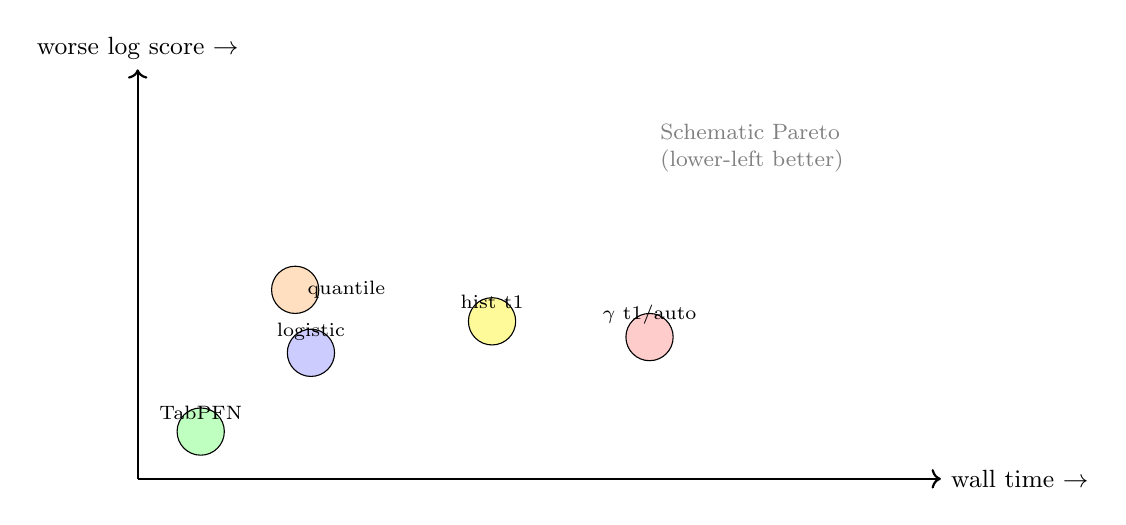
\begin{tikzpicture}[
  every node/.style={font=\small},
  m/.style={circle,draw,inner sep=1pt,minimum size=6mm}
]
\draw[->,thick] (0,0) -- (10.2,0) node[right] {wall time $\rightarrow$};
\draw[->,thick] (0,0) -- (0,5.2) node[above] {worse log score $\rightarrow$};
% schematic positions (not to scale)
\node[m,fill=green!25] (t) at (0.8,0.6) {};
\node[above=1pt] at (t) {\scriptsize TabPFN};
\node[m,fill=blue!20] (l) at (2.2,1.6) {};
\node[above=1pt] at (l) {\scriptsize logistic};
\node[m,fill=orange!25] (q) at (2.0,2.4) {};
\node[right=1pt] at (q) {\scriptsize quantile};
\node[m,fill=yellow!40] (h) at (4.5,2.0) {};
\node[above=1pt] at (h) {\scriptsize hist t1};
\node[m,fill=red!20] (g) at (6.5,1.8) {};
\node[above=1pt] at (g) {\scriptsize $\gamma$ t1/auto};
\node[font=\footnotesize,gray,align=left] at (7.8,4.2)
  {Schematic Pareto\\(lower-left better)};
\end{tikzpicture}
\caption{Schematic UQ--cost placement of active contenders (log-score axis).
Quantile sits higher on log score but is preferred when CRPS is the target.}
\label{fig:pareto}
\end{figure}

%==============================================================================
\section{When to use which model}
\label{sec:usecases}
%==============================================================================

\paragraph{TabPFN-3.5.}
Default whenever a pretrained tabular prior is allowed and the goal is
log score / CRPS / coverage jointly at minimal latency.

\paragraph{Logistic-GP (\texttt{logistic\_gp} / \texttt{logistic\_gp\_sorf\_map}).}
Classical density model of choice: $x$-separated regimes (A02), flexible
shapes without a midline, and auditable GP components. Prefer MAP$+$frozen
amplitude; do not ship VI as default.

\paragraph{Quantile GP.}
When CRPS (or pinball) is the contractual score and densities / tails are
secondary. Use GPD tails; prefer \texttt{\_hybrid\_auto} if log score also
matters. Independent-$\tau$ often wins CRPS on smooth problems; Kronecker
increments help when shape is stable in $x$.

\paragraph{MidlineSparse gamma (\texttt{\_t1} / lean auto).}
Co-located multimodality with need for expert offsets and sparsity reports.
Always standardize; always calibrate temperature (in-loop preferred). Use
\texttt{het} / auto-het when heteroscedasticity is expected (A06). Prefer
\texttt{\_1mid} or \texttt{conf\_min=0.85} until multi-midline acceptance is
revalidated. Do not expect to close the concrete RMSE gap without a stronger
Stage~1 mean.

\paragraph{hist-MoGP Tier~1.}
Keep as a classical bar-PPD control matched to TabPFN's output interface.
Not recommended as the primary hist-side contender once logistic-GP exists.

%==============================================================================
\section{Structural gaps that remain}
\label{sec:gaps}
%==============================================================================

\begin{enumerate}[leftmargin=1.4em,itemsep=0.2em]
  \item \textbf{Concrete / fish midline quality.} RMSE $\sim$5.4--6.7 vs TabPFN
        $\sim$3.7; Stage~2 cannot fix a weak midline.
  \item \textbf{A02 regime structure.} Multi-midline closes part of the gap;
        TabPFN still $\sim$0.1--0.3\,nats ahead of the best classical density.
  \item \textbf{A06 variance shape.} Homoscedastic Stage~1$+$scalar $T$ is
        insufficient; het helps but overfits on small $n$ without selection.
  \item \textbf{Quantile density.} Pinball $\neq$ NLL; hybrid $\lambda$ helps
        but does not match logistic-GP log scores.
  \item \textbf{Cost at scale.} Exact / multi-midline gamma is minutes at
        $n\sim 10^3$; SORF reduces the constant but FM latency remains an
        order of magnitude lower.
\end{enumerate}

%==============================================================================
\section{Recommendations}
\label{sec:recs}
%==============================================================================

\begin{enumerate}[leftmargin=1.4em,itemsep=0.25em]
  \item Report \textbf{TabPFN-3.5} as the FM reference on every plot/table.
  \item Make \textbf{\texttt{logistic\_gp\_sorf\_map}} the main classical
        density baseline; retire \texttt{hist\_lmc}, raw hist, and
        \texttt{hist\_gpd} from default model lists.
  \item Keep \textbf{\texttt{quantile\_gp\_sorf} / \texttt{\_hybrid\_auto}} as
        the CRPS specialists.
  \item Ship \textbf{calibrated MidlineSparse} (std$+$in-loop $T$, optional
        het, conservative multi-midline) when interpretability of modes is
        required.
  \item Always report \textbf{exact CRPS} (\texttt{CRPS\_bar} / Grimit) for
        bar and mixture models.
  \item Document negative results: VI$<$MAP, $\lambda{=}1$ hybrid overfits,
        variance expansion, learned-feature LOO means, Yu-SORF at low $d$.
\end{enumerate}

%==============================================================================
\section*{References and companion notes}
\begin{itemize}[leftmargin=1.4em,itemsep=0.15em]
  \item \texttt{docs/gamma\_mlp\_hist\_mogp\_analysis.md} --- Tier 1--4 narrative
        and novelty assessment.
  \item \texttt{docs/midline\_sparse\_pipeline.tex} --- MidlineSparse
        pipeline derivations.
  \item \texttt{docs/midline\_sparse\_probabilistic\_foundations.tex} ---
        EB--MAP vs Bayesian status of the MoG predictive.
  \item \texttt{docs/midline\_siblings\_and\_hist\_gp.tex} --- residual/Bayes
        MoGP siblings and hist baselines.
  \item Result tables:
        \texttt{results/foundation\_compare\_tier\{1,3,4\}/summary\_table.md}.
\end{itemize}

\begin{thebibliography}{99}
\bibitem{foundations-note}
SpectralGPPlus technical note.
\textit{What Prior Does MidlineSparse Impose?}
\texttt{docs/midline\_sparse\_probabilistic\_foundations.tex}.

\bibitem{louizos2018}
C.~Louizos, M.~Welling, D.~P.~Kingma.
Learning sparse neural networks through $L_0$ regularization.
\textit{ICLR}, 2018.

\bibitem{grimit2006}
E.~P.~Grimit, T.~Gneiting, V.~J.~Berrocal, N.~A.~Johnson.
The continuous ranked probability score for circular variables.
\textit{Q.\ J.\ R.\ Meteorol.\ Soc.}, 2006.

\bibitem{yu2016}
F.~X.~X.~Yu et al.
Orthogonal random features.
\textit{NeurIPS}, 2016.

\bibitem{tokdar2010}
S.~T.~Tokdar, Y.~M.~Zhu, J.~K.~Ghosh.
Bayesian density regression with logistic Gaussian process.
\textit{Bayesian Analysis}, 2010.

\bibitem{abeywardana2015}
S.~Abeywardana, F.~Ramos.
Variational inference for nonparametric Bayesian quantile regression.
\textit{AAAI}, 2015.

\bibitem{bishop1994}
C.~M.~Bishop.
Mixture density networks.
Aston University technical report NCRG/94/004, 1994.
\end{thebibliography}

\end{document}
